%----------------------------------------------------------------------------------------
%	PACKAGES AND OTHER DOCUMENT CONFIGURATIONS
%----------------------------------------------------------------------------------------

\documentclass[paper=a4, fontsize=11pt]{scrartcl} % A4 paper and 11pt font size

\usepackage[margin=1.0in]{geometry}	%for some reason, looks beter. 

\usepackage[T1]{fontenc} % Use 8-bit encoding that has 256 glyphs
\usepackage{fourier} % Use the Adobe Utopia font for the document - comment this line to return to the LaTeX default
\usepackage[english]{babel} % English language/hyphenation
\usepackage{amsmath,amsfonts,amsthm} % Math packages

\usepackage{lipsum} % Used for inserting dummy 'Lorem ipsum' text into the template

\usepackage{sectsty} % Allows customizing section commands
\allsectionsfont{\centering \normalfont\scshape} % Make all sections centered, the default font and small caps

\usepackage{fancyhdr} % Custom headers and footers
\pagestyle{fancyplain} % Makes all pages in the document conform to the custom headers and footers
\fancyhead{} % No page header - if you want one, create it in the same way as the footers below
\fancyfoot[L]{} % Empty left footer
\fancyfoot[C]{} % Empty center footer
\fancyfoot[R]{\thepage} % Page numbering for right footer
\renewcommand{\headrulewidth}{0pt} % Remove header underlines
\renewcommand{\footrulewidth}{0pt} % Remove footer underlines
\setlength{\headheight}{13.6pt} % Customize the height of the header

\numberwithin{equation}{section} % Number equations within sections (i.e. 1.1, 1.2, 2.1, 2.2 instead of 1, 2, 3, 4)
\numberwithin{figure}{section} % Number figures within sections (i.e. 1.1, 1.2, 2.1, 2.2 instead of 1, 2, 3, 4)
\numberwithin{table}{section} % Number tables within sections (i.e. 1.1, 1.2, 2.1, 2.2 instead of 1, 2, 3, 4)

\setlength\parindent{0pt} % Removes all indentation from paragraphs - comment this line for an assignment with lots of text

%----------------------------------------------------------------------------------------
%Personal Packages and File Dependencies 
%----------------------------------------------------------------------------------------	

\usepackage{graphicx}	%insert graphics
\usepackage{microtype}	%improves spacing
\usepackage{float}		%H postion	
\usepackage{caption}	%caption w/o : 	
\usepackage{framed}		%creates frames
\usepackage{enumitem}
\usepackage{nag}

\usepackage{listings}	%insert sourcecode
\usepackage{color}
\usepackage{pdfpages}	%include PDF pages

\usepackage{bigstrut}	%exce2latex table packages
\usepackage{rotating}
\usepackage{multirow}
\usepackage{booktabs}
%\usepackage[framed]{mcode}

\usepackage{cleveref}	%cooler references, needs to be last
\usepackage[bookmarks]{hyperref}
\graphicspath{{../Figures/}{../figures/}} % This automatically connects to the figure folder

%----------------------------------------------------------------------------------------
%	TITLE SECTION
%----------------------------------------------------------------------------------------

\newcommand{\horrule}[1]{\rule{\linewidth}{#1}} % Create horizontal rule command with 1 argument of height

\title{	
\normalfont \normalsize 
\textsc{TEMPLE UNIVERSITY COLLEGE OF ENGINEERING | ECE 3623 | SPRING 2015} \\ [25pt] % Your university, school and/or department name(s)
\horrule{0.5pt} \\[0.4cm] % Thin top horizontal rule
\huge Embedded Systems Lab 1: Regression and Histograms \\ % The assignment title
\horrule{2pt} \\[0.5cm] % Thick bottom horizontal rule
}

\author{Tyler Berezowsky} % Your name

\date{\normalsize\today} % Today's date or a custom date 
\usepackage[]{listing}
\lstset{language=Python}
\lstset{literate=
  {á}{{\'a}}1 {é}{{\'e}}1 {í}{{\'i}}1 {ó}{{\'o}}1 {ú}{{\'u}}1
  {Á}{{\'A}}1 {É}{{\'E}}1 {Í}{{\'I}}1 {Ó}{{\'O}}1 {Ú}{{\'U}}1
  {à}{{\`a}}1 {è}{{\`e}}1 {ì}{{\`i}}1 {ò}{{\`o}}1 {ù}{{\`u}}1
  {À}{{\`A}}1 {È}{{\'E}}1 {Ì}{{\`I}}1 {Ò}{{\`O}}1 {Ù}{{\`U}}1
  {ä}{{\"a}}1 {ë}{{\"e}}1 {ï}{{\"i}}1 {ö}{{\"o}}1 {ü}{{\"u}}1
  {Ä}{{\"A}}1 {Ë}{{\"E}}1 {Ï}{{\"I}}1 {Ö}{{\"O}}1 {Ü}{{\"U}}1
  {â}{{\^a}}1 {ê}{{\^e}}1 {î}{{\^i}}1 {ô}{{\^o}}1 {û}{{\^u}}1
  {Â}{{\^A}}1 {Ê}{{\^E}}1 {Î}{{\^I}}1 {Ô}{{\^O}}1 {Û}{{\^U}}1
  {œ}{{\oe}}1 {Œ}{{\OE}}1 {æ}{{\ae}}1 {Æ}{{\AE}}1 {ß}{{\ss}}1
  {ç}{{\c c}}1 {Ç}{{\c C}}1 {ø}{{\o}}1 {å}{{\r a}}1 {Å}{{\r A}}1
  {€}{{\EUR}}1 {£}{{\pounds}}1
}

\begin{document}
\maketitle % Print the title

\section{Problem Statement} 
%Summarize the problem statement in one paragraph. Clearly state what the knowns are and what unknowns you must find.
Use MATLAB's random number generator and generate uniformly distributed random numbers on the range $[0,1]$. We all agree that the mean, $\mu$, should be $0.5$, and the variance, $\sigma^2$, should be ??? (can you derive this?).
The tasks to be accomplished are:
\begin{enumerate}
\item  Generate N random numbers, denoted by the signal $x[n]$. Estimate the mean (equation~\ref{eq: mean}) and variance (equation~\ref{eq: variance}) using N data points. Compute the error of these estimates as:
$E_{\tilde{\mu}}[N] = \tilde{\mu_X}[N] - \mu$ and $E_{\tilde{\sigma}}[N] = \tilde{\sigma}^2_X[N] - \sigma^2$. 
\begin{equation} 
\tilde{\mu}_x[N] = \frac{1}{n}\sum_{n=0}^{N-1} x[N]
\label{eq: mean}
\end{equation}
\begin{equation}
\tilde{\sigma}^2[N] = \frac{1}{N}\sum_{n=0}^{N-1}(x[n]-\tilde{\mu})^2
\label{eq: variance}
\end{equation}

Plot $E_{\tilde{\mu}}[N]$ and $E_{\tilde{\mu}}[N]$ for $N=[1, 1e6]$. Use a log base 10 scale for the horizontal axis (n - the number of points) and a linear scale for the error. Explain this plot.
\item  Estimate the pdf of $x[n]$ using a bin size of 0.01 (100 bins for the range $[0,1]$). Plot the mean-squared error between the measured distribution and the actual distribution using:
\begin{equation}
MSE = \frac{1}{B}\sum_{b=0}^{B-1}[\tilde{p}_X(x)-p(x)]^2
\label{eq: mse}
\end{equation}

where B is the number of bins, $p(x)$ is the ``true'' distribution (a uniform distribution in this case), and  is the estimate of the distribution. Obviously, for $N < B$, some of the bins will be empty. Does that remind you of the exam problem?
Estimate the pdf for $N = [1, 1e6]$, and plot $MSE[N]$ using the same linear/log scale as above. Explain your findings. Plot the pdfs for N = 101, 103, and 106 and compare/contrast them.
\end{enumerate}

\section{Approach and Results} 
%Describe your approach to finding the unknowns. Use numbered figures, tables and equations where necessary.
A uniform distribution is described by equation~\ref{eq: uniform} below. The variance of a uniform distribution was calculated by finding the second moment of the distribution and subtracting it from the first squared. The result is displayed below.  
\begin{equation}
p_X(x) = \left\{ 
	\begin{array}{lcr}
		\frac{1}{b-a} & : & a \leq x \leq b \\
		0 & : & otherwise
	\end{array} 
	\right.
\label{eq: uniform}
\end{equation}
\begin{equation}
\sigma^2_X= E[X]^2 - E[X^2] = \frac{1}{2}(b + a) - \int_{a}^b x^2p_x(x)dx = \frac{1}{12}(b - a)^2
\end{equation}

Instead of utilizing MATLAB for calculations, python coupled with numpy and matplotlib was utilized. The script \verb|ca_06.py| generates a random uniformly distributed vector ($x$) of $1\times10^6$ samples. Equations~\ref{eq: mean} to \ref{eq: mse} are then run on the vector. The results are stored to file. An additional script was written, \verb|ca_06_publishing.py|, to load the data, generate the requested histograms, and the error plots. The scripts were separated to run the bulk of the calculation on the electrodata server provided by Temple. \\

The results are listed below. Figures~\ref{fig: meanerror} to \ref{fig: mse} display the error between the estimated mean, variance and pdf, and their actual  values for a uniform distribution. The abscissa is base-10 logarithmically scaled and represents the number of samples taken from $x$ for the calculated. The error for figure~\ref{fig: meanerror} and figure~\ref{fig: varerror} is scaled linearly. The MSE between the estimated and expected pdf is scaled logarithmically. \\


\begin{figure}[H] 
	\centering 
	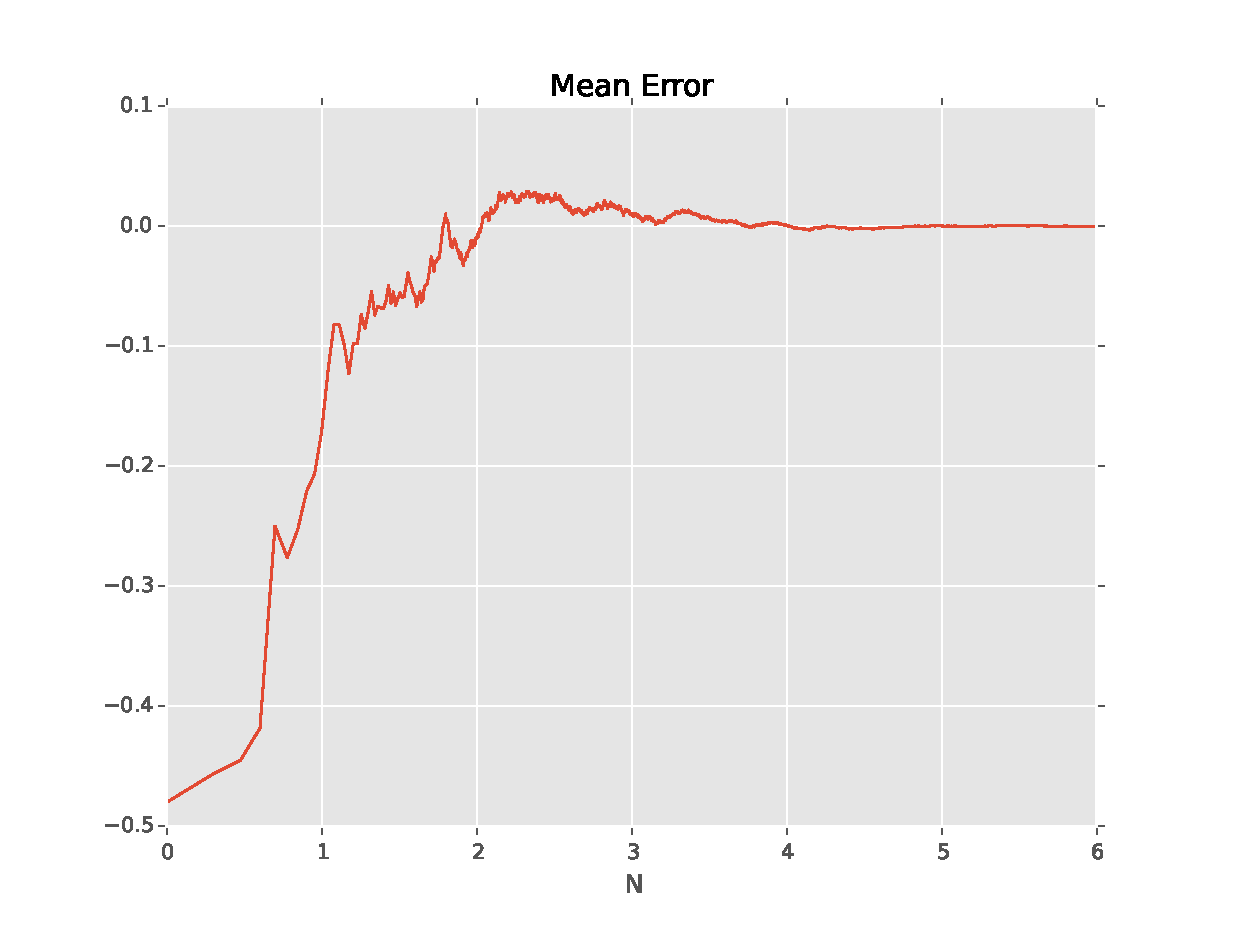
\includegraphics[width=\linewidth]{figure_1}
	\caption{$Err[\tilde{\mu}_X](N)$, $N = [1, 1e6]$}
	\label{fig: meanerror} 
\end{figure}

\begin{figure}[H] 
	\centering 
	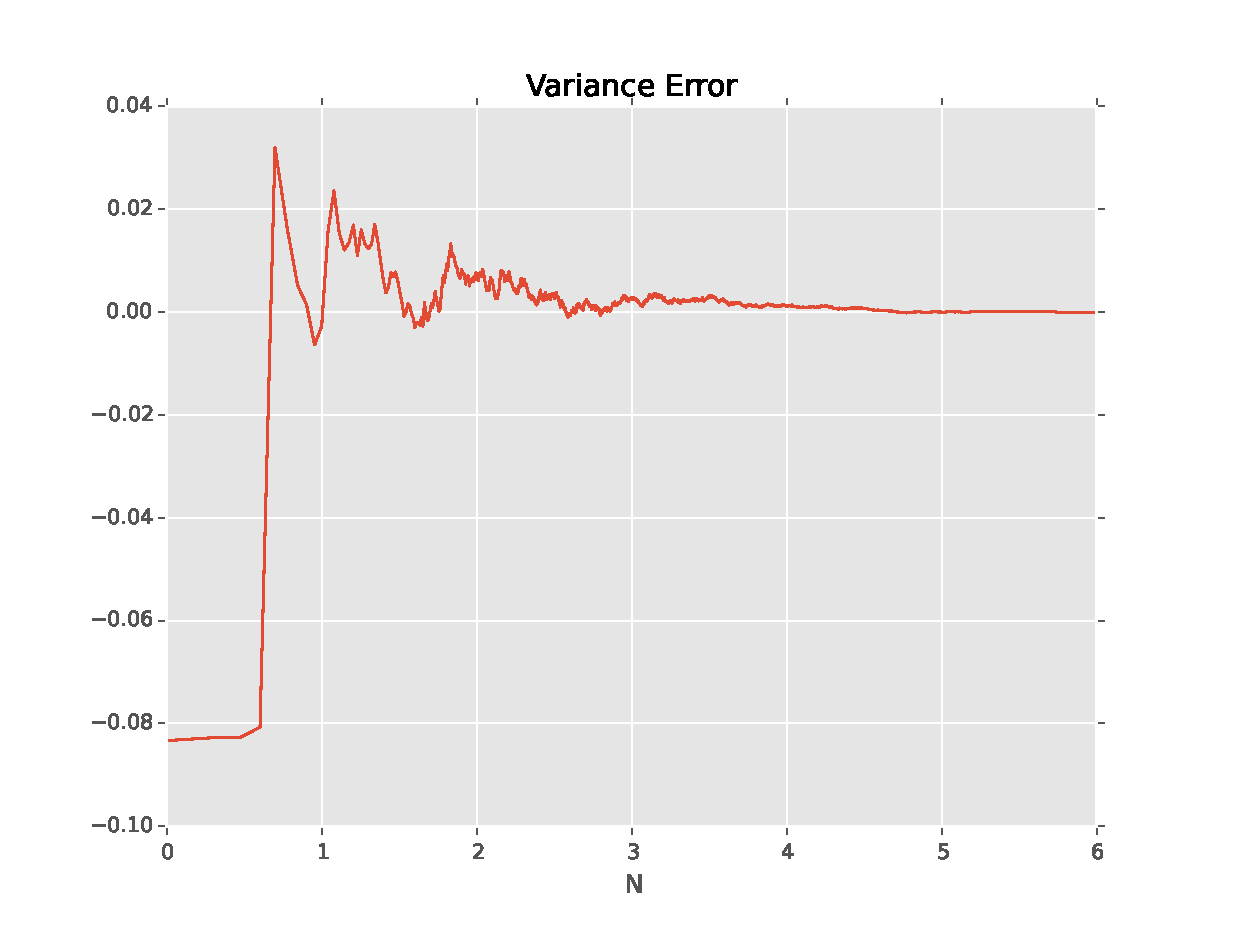
\includegraphics[width=\linewidth]{figure_2}
	\caption{$Err[\tilde{\sigma}^2_X](N)$, $N = [1, 1e6]$}
	\label{fig: varerror} 
\end{figure}

\begin{figure}[H] 
	\centering 
	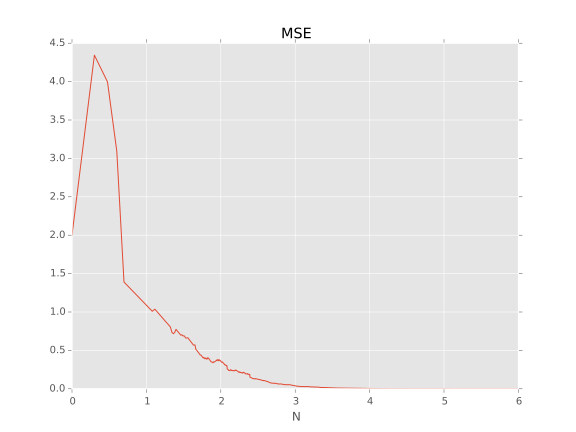
\includegraphics[width=\linewidth]{figure_3}
	\caption{$Err[MSE](N)$, $N = [1, 1e6]$}
	\label{fig: mse} 
\end{figure}

Figure~\ref{fig: hist} below illustrates the histogram or pdf of the data when 10, 1,000 and 1,000,000 samples are taken from $x$. The abscissa is represents the possible values of the vector, and the y-axis represents the probability of each value. \\


For a uniform distribution with 100 bins, the probability of each bin should be 0.01. As the number of samples increases, the histograms approach the actual distribution. This is reflected visually in the three plots below, but also through error of the metrics calculated above. As $N$ increases, the error between the metrics decrease because the sample space, with more data, is more reflective of the uniform distribution. 

\begin{figure}[H] 
	\centering 
	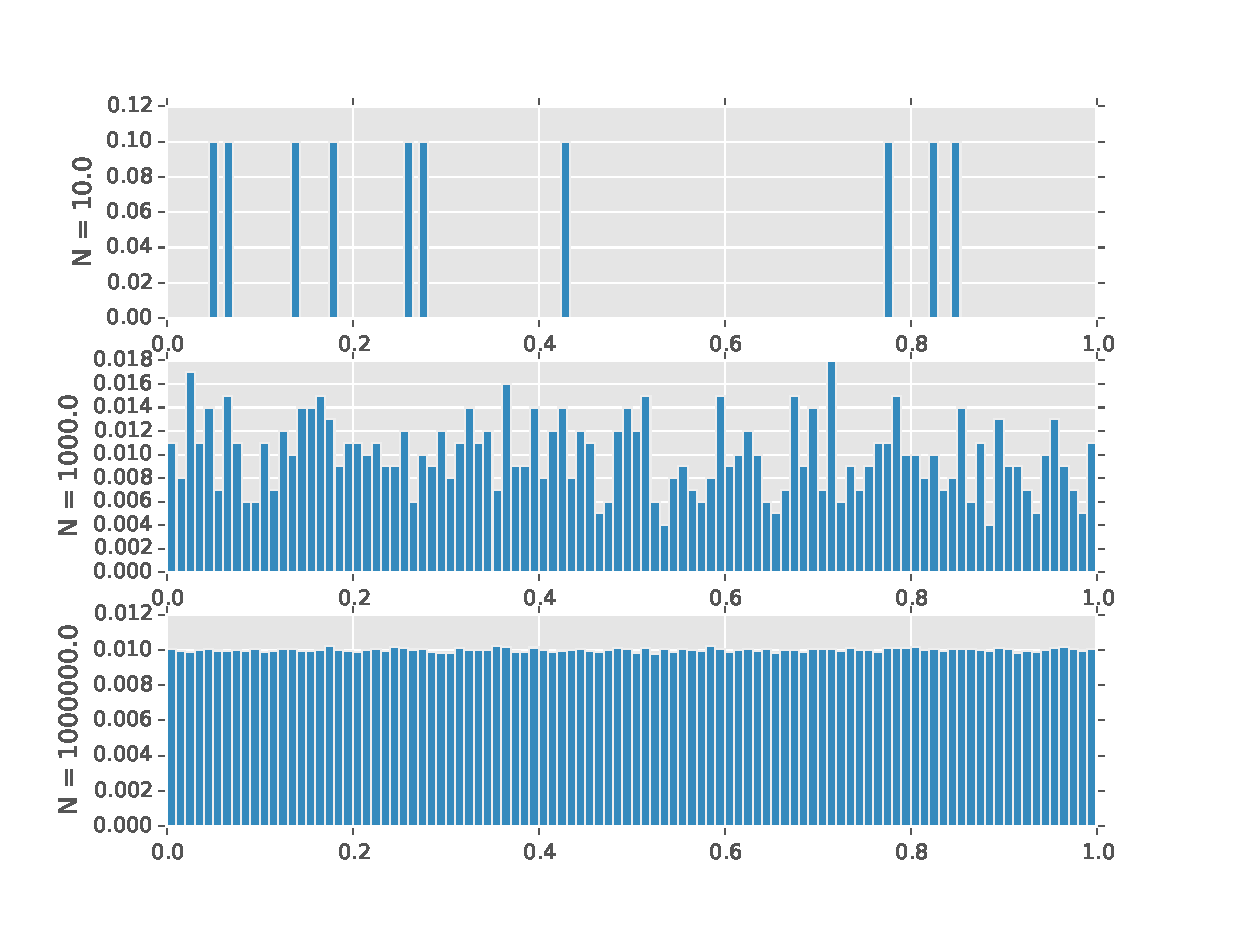
\includegraphics[width=\linewidth]{figure_4}
	\caption{Histogram of random uniform distributed vector, $p_x(N)$, of $N$ elements.}
	\label{fig: hist} 
\end{figure}

\section{Python Code} 
%Show and briefly explain your Python code.
\lstinputlisting[frame=single]{../Python/ca_06.py}
\lstinputlisting[frame=single]{../Python/ca_06_publishing.py}

\section{Conclusions} 
%Summarize what you found.
As a sample space increases with valid data, the space better reflects its governing distribution. This is clearly illustrated through the histograms and the three error plots. Therefore, if the sample space is not sufficiently large any metrics calculated to represent the space would not reflect the governing distribution.  

\end{document}